% Created 2014-07-21 Mon 22:11
\documentclass[utf8x,notes,17pt]{beamer}
\usepackage[T1]{fontenc}
\usepackage{fixltx2e}
\usepackage{graphicx}
\usepackage{longtable}
\usepackage{float}
\usepackage{wrapfig}
\usepackage{rotating}
\usepackage[normalem]{ulem}
\usepackage{amsmath}
\usepackage{textcomp}
\usepackage{marvosym}
\usepackage{wasysym}
\usepackage{amssymb}
\usepackage{hyperref}
\tolerance=1000
\setbeamertemplate{navigation symbols}{}
\usepackage{courier}
\usepackage{helvet}
\usepackage{listings}
\usepackage{mathtools}
\usepackage{pdfcomment}
\SetUnicodeOption{mathletters}
\DeclareUnicodeCharacter{952}{\theta}
\lstset{
keywordstyle=\color{blue}
, basicstyle=\ttfamily\small
, commentstyle={}
, columns=fullflexible
, showstringspaces=false
, keepspaces=true=
, breaklines=true
, escapeinside={\%*}{*)},
}
\newcommand{\head}[1]{\begin{center}
\vspace{13mm}\hspace{-1mm}\Huge{{#1}}
\end{center}}
\renewcommand{\note}[1]{\marginnote{\pdfcomment[icon=note]{#1}}}
\usetheme[height=16mm]{Rochester}
\author{John Wiegley}
\date{22 Jul 2014}
\title{Monads and other abstractions}
\hypersetup{
  pdfkeywords={math monad haskell functional programming},
  pdfsubject={Applying mathematical abstractions to functional programming},
  pdfcreator={Emacs 24.3.1 (Org mode 8.2.6)}}
\begin{document}

\maketitle
\setbeamertemplate{footline}{}
\setbeamerfont{block body}{size=\small}
\definecolor{orchid}{RGB}{134, 134, 220}
\setbeamercolor{block title}{fg=white,bg=orchid}
\setbeamercolor{bgcolor}{fg=white,bg=blue}

\section{Overview}
\label{sec-1}
\begin{frame}[fragile,label=sec-1-1]{Workshop overview}
\begin{enumerate}
\item Basic math definitions
\item Algebras and laws
\item Working with proofs
\item Category theory \& Functors
\item Monads
\end{enumerate}
\note{note
Give an introduction of myself and my background here, and ask whether people
in the audience have much experience with the intersection between math and
programming.}
\end{frame}
\section{Mathematics}
\label{sec-2}
\begin{frame}[fragile,plain,label=sec-2-1]{HEAD}
\head{Mathematics}
\end{frame}
\begin{frame}[fragile,label=sec-2-2]{Meaning}
There isn't any.
\note{note
One of the things that tripped me up most when I started studying math was my
desire for meaning: for examples that would motivate and explain what the
concept was "about" or "for".}
\end{frame}
\begin{frame}[fragile,label=sec-2-3]{Abstraction}
Structures, and relationships between structures.
\note{note
Math is really a language, a whole system, for talking about structures and
their relationships.  Meaning and abstraction form a kind of tension, since
you move away from meaning into abstraction, and to gain meaning you must give
up abstraction.}
\end{frame}
\section{Sets}
\label{sec-3}
\begin{frame}[fragile,plain,label=sec-3-1]{HEAD}
\head{Sets}
\note{note
What is really interesting is just how much can be done with such a minimal
amount of structure.}
\end{frame}
\begin{frame}[fragile,label=sec-3-2]{``Stuff''}
\begin{center}
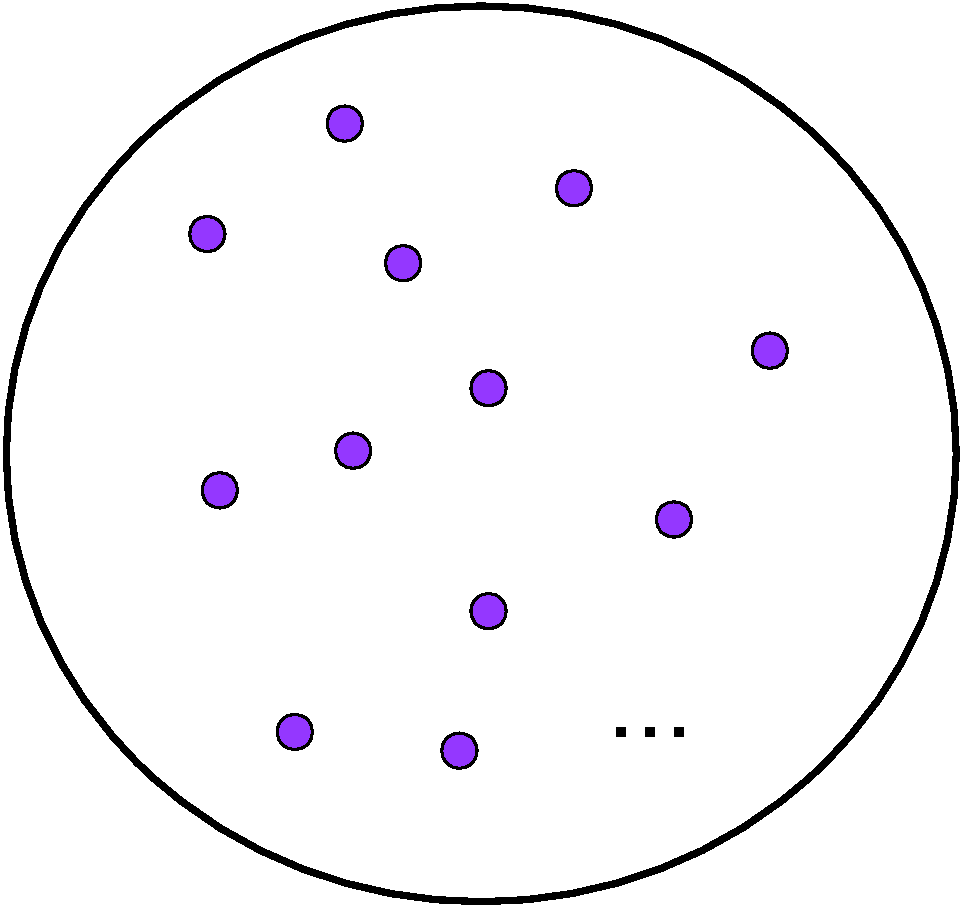
\includegraphics[width=.65\linewidth]{images/Sets1.pdf}
\end{center}
\end{frame}
\begin{frame}[fragile,label=sec-3-3]{``Stuff''}
\begin{center}
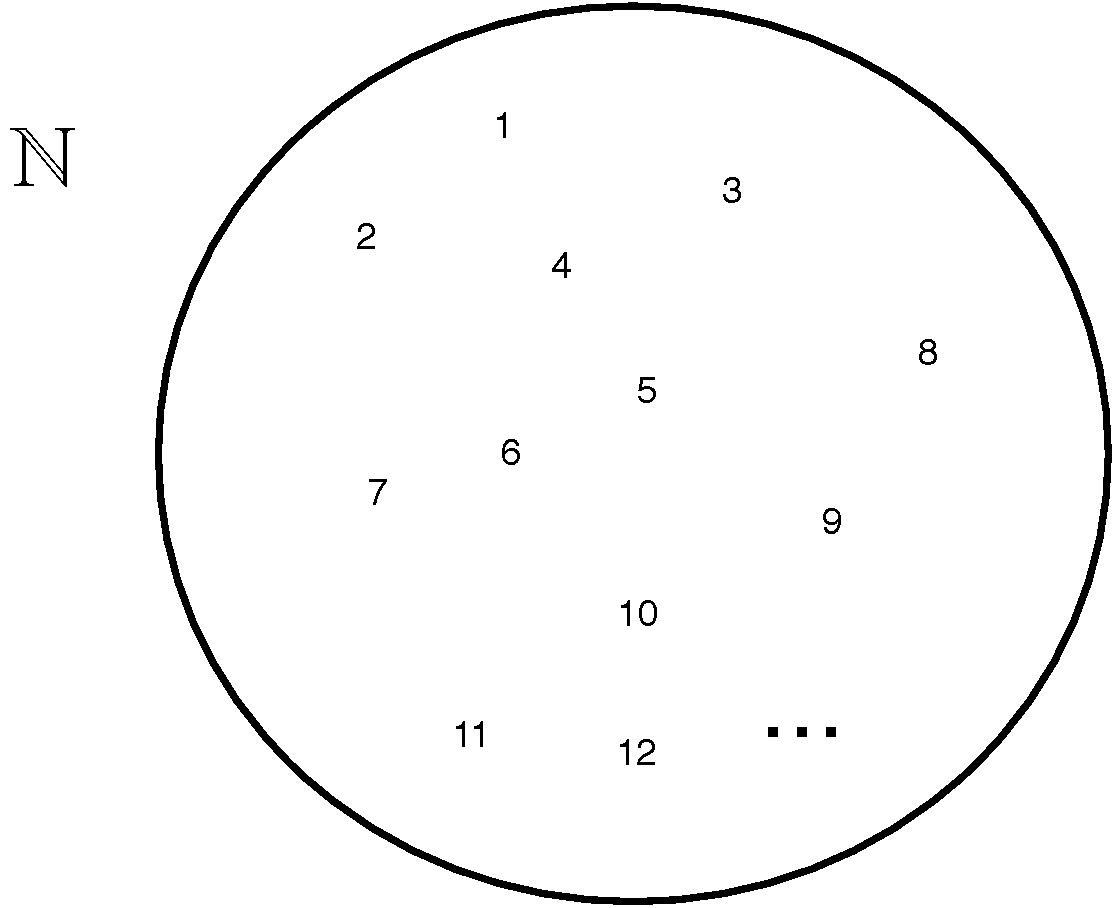
\includegraphics[width=.65\linewidth]{images/Sets2.pdf}
\end{center}
\end{frame}
\begin{frame}[fragile,label=sec-3-4]{Sets of sets}
\begin{center}
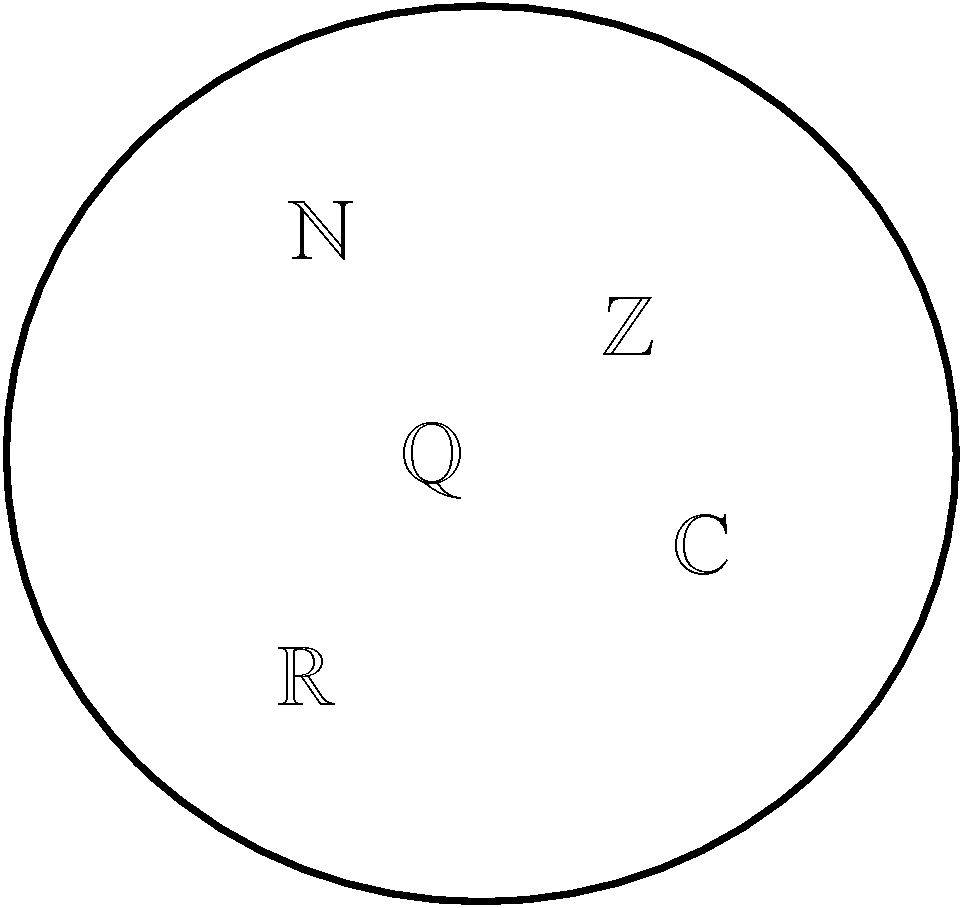
\includegraphics[width=.65\linewidth]{images/Sets3.pdf}
\end{center}
\end{frame}
\begin{frame}[fragile,label=sec-3-5]{Extensional}
Can be defined by stating its elements.
\begin{example}[\vspace*{-3.5ex}]
\( \{ \ True, False\ \} \)
\end{example}
\end{frame}
\begin{frame}[fragile,label=sec-3-6]{Intensional}
Or by describing them.
\begin{example}[\vspace*{-3.5ex}]
\( \{ \ x \ |\  x \in \mathbb{N}, even(x)\ \} \)
\end{example}
\end{frame}
\begin{frame}[fragile,label=sec-3-7]{Programmatic}
Can be modeled programmatically.
\begin{example}[\vspace*{-3.5ex}]
\begin{lstlisting}[language=Haskell]
type Set a = a -> Bool

import Data.Set as S
type Set a = S.Set a
\end{lstlisting}
\end{example}
\note{note
This introduces the idea of modeling constructs as functions instead of data
structures.}
\end{frame}
\begin{frame}[fragile,label=sec-3-8]{Exercise}
Using the functional definition of sets, define union and intersection.
\begin{alertblock}{\vspace*{-3.5ex}}
\begin{lstlisting}[language=Haskell]
type Set a = a -> Bool

union :: Set a -> Set a -> Set a
inter :: Set a -> Set a -> Set a
\end{lstlisting}
\end{alertblock}
\end{frame}
\begin{frame}[fragile,label=sec-3-9]{Deceptively simple}
With a basic definition and seven axioms (we've seen two!), you can generate a
good deal of mathematics.
\end{frame}
\section{Functions}
\label{sec-4}
\begin{frame}[fragile,plain,label=sec-4-1]{HEAD}
\head{Functions}
\end{frame}
\begin{frame}[fragile,label=sec-4-2]{Domain, co-domain, range}
\begin{center}
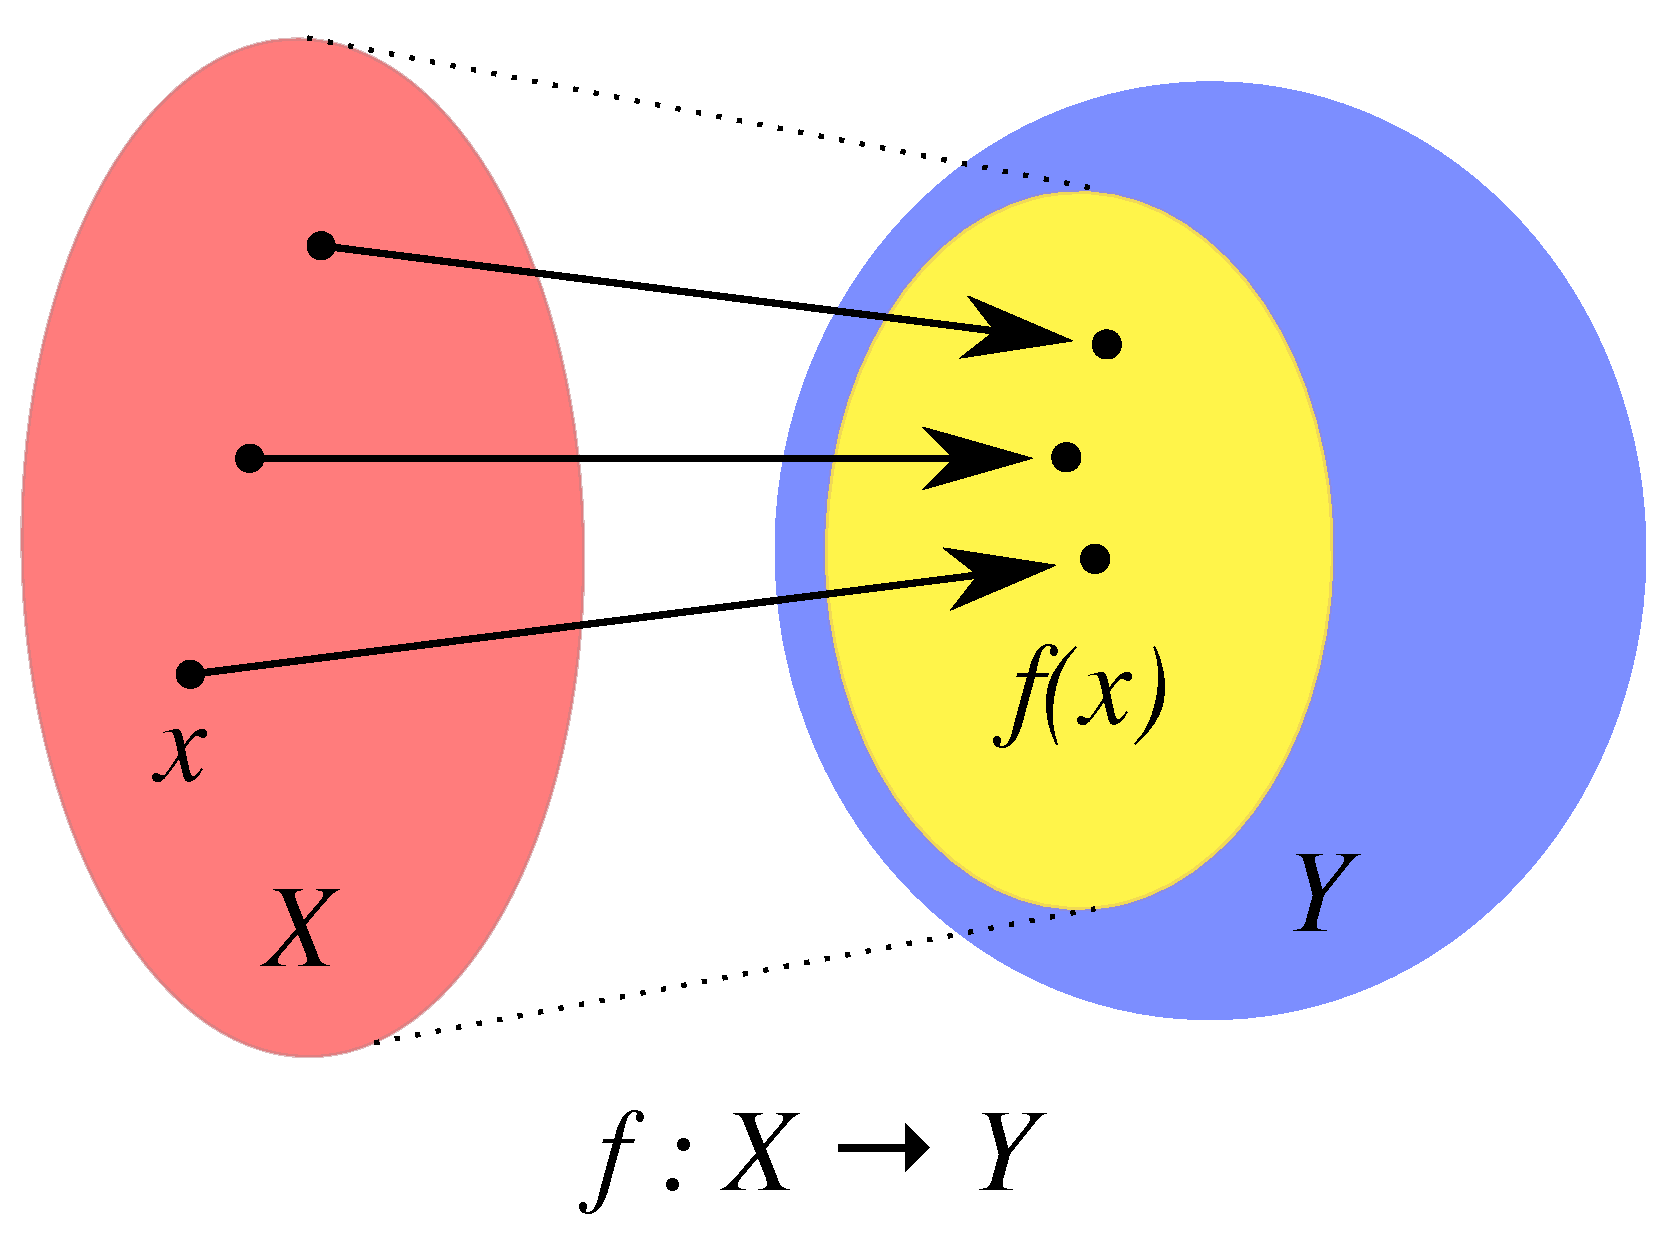
\includegraphics[width=.9\linewidth]{images/Codomain2.pdf}
\end{center}
\end{frame}
\begin{frame}[fragile,label=sec-4-3]{Injective}
\begin{center}
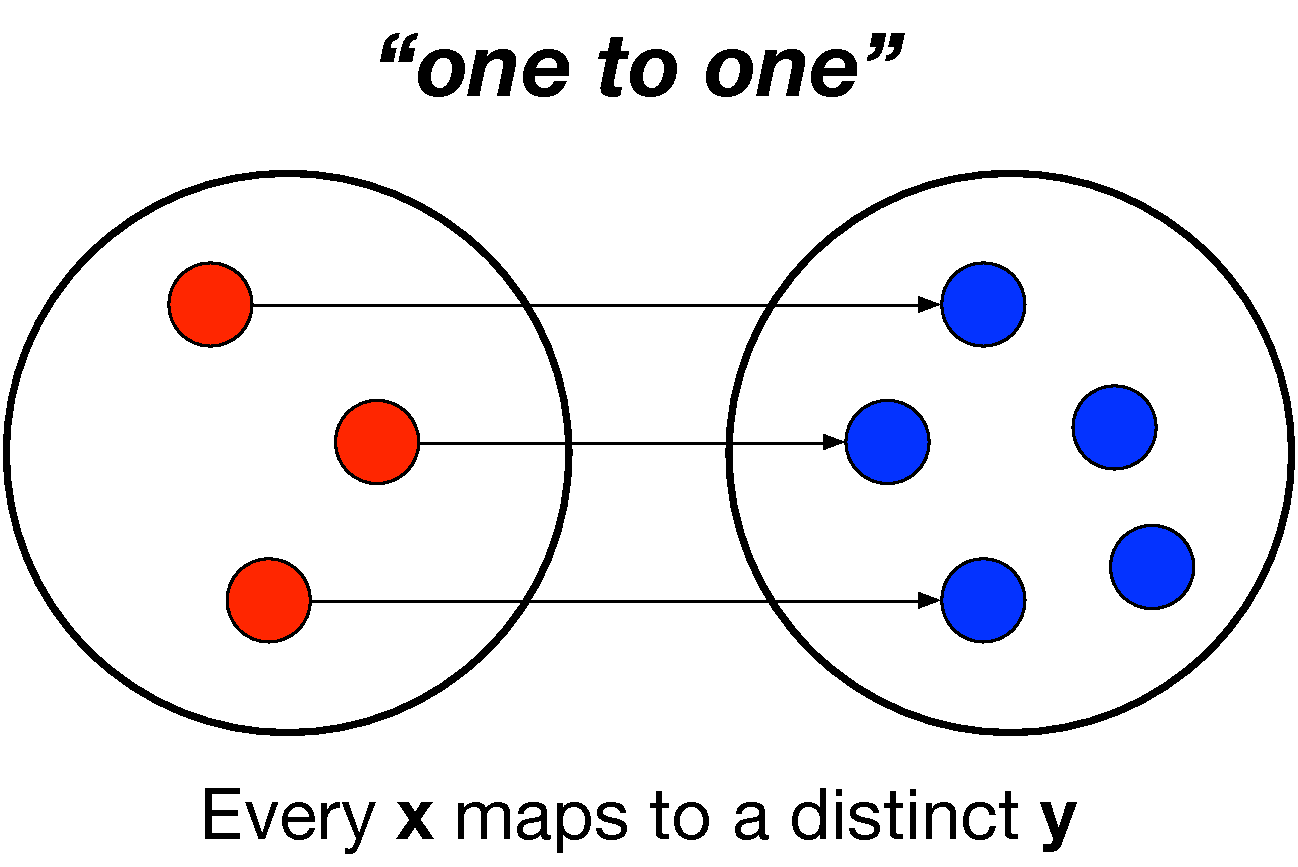
\includegraphics[width=.9\linewidth]{images/Mappings1.pdf}
\end{center}
\end{frame}
\begin{frame}[fragile,label=sec-4-4]{Injective}
\[ f : A → B \]

\[ ∀ x, y ∈ A \]

\[ f\ x = f\ y → x = y \]
\end{frame}
\begin{frame}[fragile,label=sec-4-5]{Injective}
Examples of injective things:

\begin{itemize}
\item Data constructors
\item Type constructors
\item But not type synonyms\dots{}
\end{itemize}
\end{frame}
\begin{frame}[fragile,label=sec-4-6]{Exercise}
\begin{enumerate}
\item Write an injective function on \texttt{Integer}, and one that is not
injective.

\item How do you test it in both cases?
\end{enumerate}
\end{frame}
\begin{frame}[fragile,label=sec-4-7]{Surjective}
\begin{center}
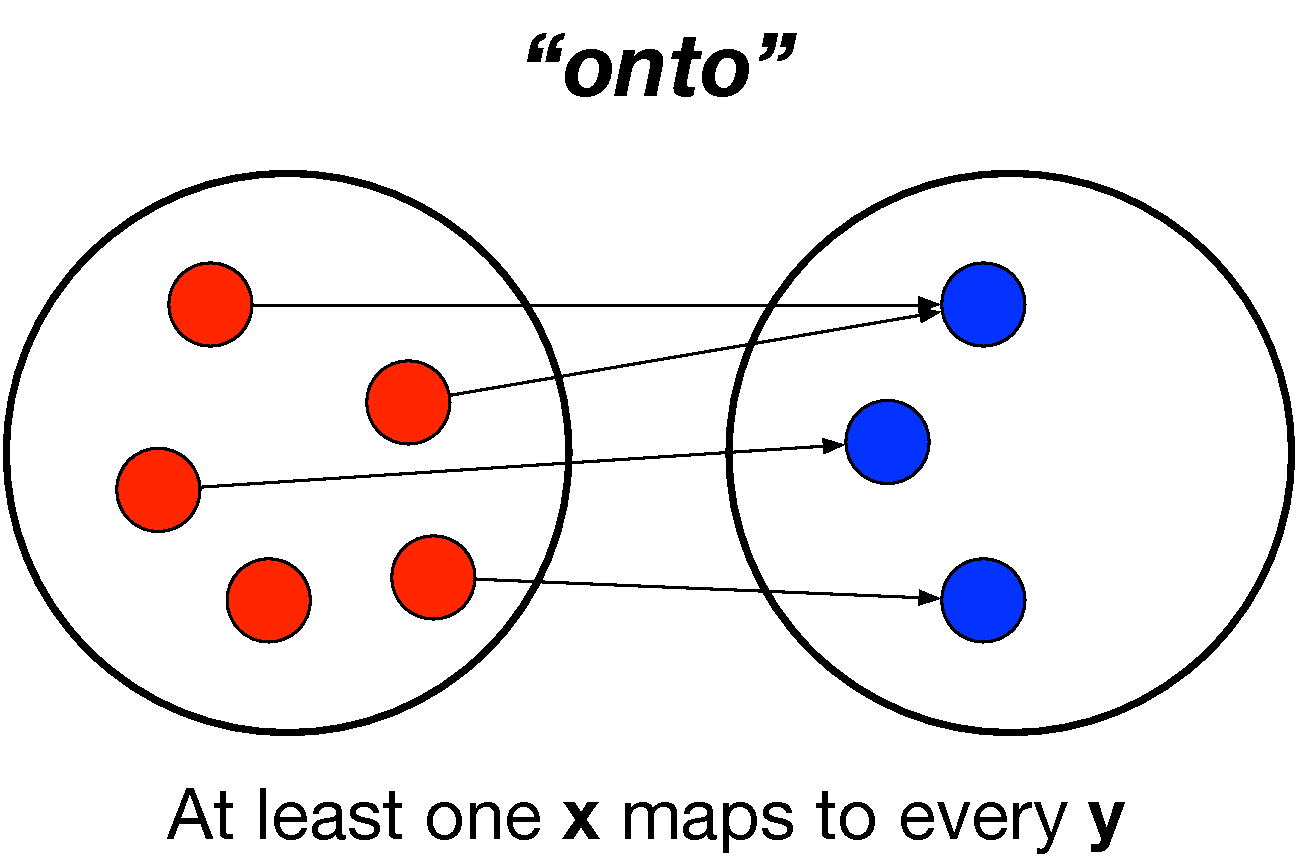
\includegraphics[width=.9\linewidth]{images/Mappings2.pdf}
\end{center}
\end{frame}
\begin{frame}[fragile,label=sec-4-8]{Surjective}
\[ f : A → B \]

\[ ∀ y ∈ B, ∃ x ∈ A \]

\[ f\ x = y \]
\end{frame}
\begin{frame}[fragile,label=sec-4-9]{Surjective}
A function is surjective if the set of possible results is not a subset of its
type.  Example:

\begin{itemize}
\item \texttt{even} is surjective
\item \texttt{times2} is not
\end{itemize}
\end{frame}
\begin{frame}[fragile,label=sec-4-10]{Bijective}
\begin{center}
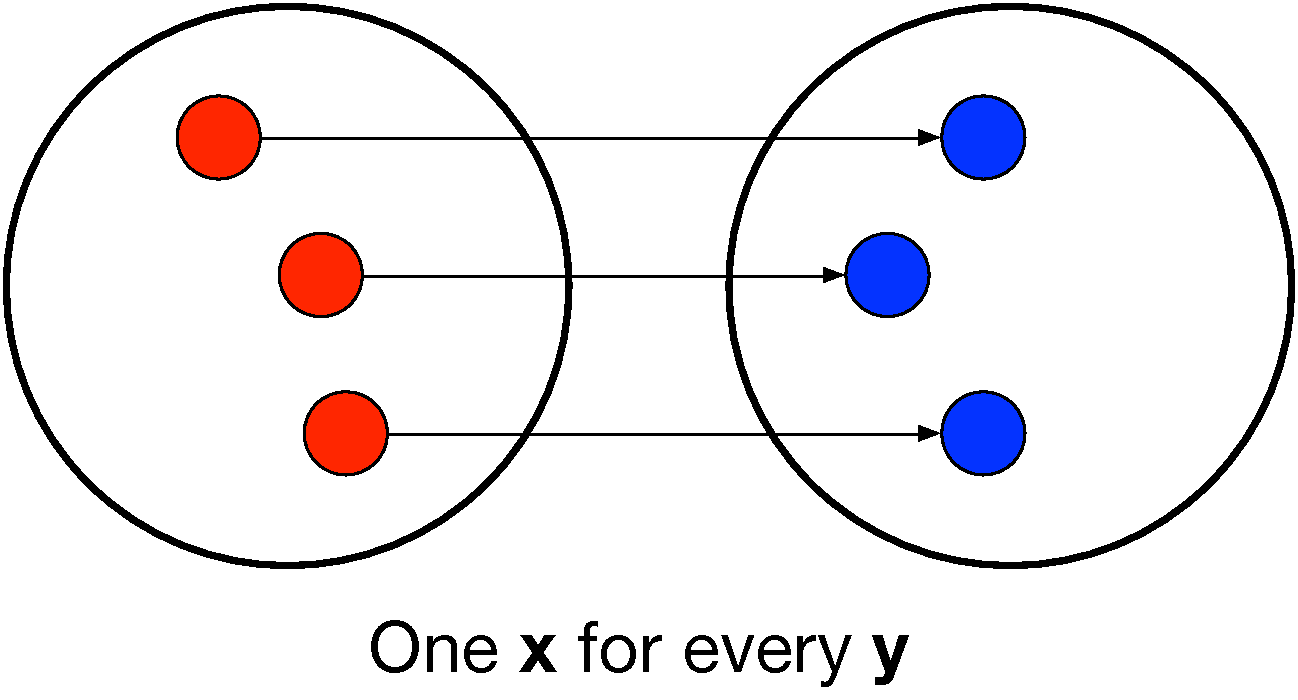
\includegraphics[width=.9\linewidth]{images/Mappings3.pdf}
\end{center}
\end{frame}
\begin{frame}[fragile,label=sec-4-11]{Higher-order functions}
\begin{definition}[Identity]
\( id\ x = x \)
\end{definition}
\begin{definition}<2->[Composition]
\( (f ∘ g)\ x = f (g(x)) \)
\end{definition}
\end{frame}
\begin{frame}[fragile,label=sec-4-12]{Properties of functions}
\[ f : dom → cod \]
\note{note
A powerful concept is to define properties of functions in terms of functions
and equalities.}
\begin{definition}<2->[Idempotent]
\( f ∘ f = f \)
\end{definition}
\begin{definition}<3->[Involutive]
\( f ∘ f = id \)
\end{definition}
\end{frame}
\begin{frame}[fragile,label=sec-4-13]{More properties}
\begin{definition}[Section]
\( f ∘ s = id \)
\end{definition}
\begin{definition}[Retract]
\( r ∘ f = id \)
\end{definition}
\note{note
I only mention these to show how much structures we can infer from a very
small set of building blocks.}
\end{frame}
\begin{frame}[fragile,label=sec-4-14]{Exercise}
For the set of integers, show examples of:

\begin{enumerate}
\item idempotency
\item involution
\item section
\item retraction
\end{enumerate}
\end{frame}
\begin{frame}[fragile,label=sec-4-15]{Isomorphism}
An isomorphism is a pair of functions satisfying two equations:

\[ f ∘ g = id_{cod(f)} \]
\[ g ∘ f = id_{cod(g)} \]
\end{frame}
\begin{frame}[fragile,label=sec-4-16]{Isomorphism}
In terms of the types involved:

\[ A ≅ B \]

\[ g : A → B \]
\[ f : B → A \]
\note{note
Assuming of course \( cod(f) = A, cod(g) = B \).}
\end{frame}
\begin{frame}[fragile,label=sec-4-17]{Exercise}
\vspace{-2ex}
\begin{example}[\vspace*{-3.5ex}]
\begin{lstlisting}[language=Haskell]
data Unit = Unit
data Maybe a = Nothing | Just a
\end{lstlisting}
\end{example}
\begin{alertblock}<2->{Write two functions}
\fontsize{14}{16}\selectfont
\vspace{-2ex}
\begin{align*}
\texttt{toMaybe}   & :: \texttt{Integer}\ →\ \texttt{Maybe\ Unit} \\
\texttt{fromMaybe} & :: \texttt{Maybe\ Unit}\ →\ \texttt{Integer}
\end{align*}
\end{alertblock}
\end{frame}
\section{Laws}
\label{sec-5}
\begin{frame}[fragile,plain,label=sec-5-1]{HEAD}
\head{Laws}
\end{frame}
\begin{frame}[fragile,label=sec-5-2]{Imposed structure}
In the absence of meaning, laws create structure.
\end{frame}
\begin{frame}[fragile,label=sec-5-3]{Principled restriction}
Laws restrict how functions and values relate to each other.
\begin{example}<2->[\vspace*{-3.5ex}]
\begin{lstlisting}[language=Haskell]
class Monoid a where
  mempty  :: a
  mappend :: a -> a -> a
\end{lstlisting}
\end{example}
\note{note
Give the example of why mempty from Monoid is good, but point from Pointed is
not.}
\end{frame}
\begin{frame}[fragile,label=sec-5-4]{Associativity}
\[ x ∙ (y ∙ z) = (x ∙ y) ∙ z \]
\end{frame}
\begin{frame}[fragile,label=sec-5-5]{Commutativity}
\[ x ∙ y = y ∙ x \]
\end{frame}
\begin{frame}[fragile,label=sec-5-6]{Transitivity}
\[ x ∙ y → y ∙ z → x ∙ z \]
\end{frame}
\begin{frame}[fragile,label=sec-5-7]{Lawless!}
Behold, the face of evil:
\begin{example}[\vspace*{-3.5ex}]
\begin{lstlisting}[language=Haskell]
class Pointed a where
  point :: a
\end{lstlisting}
\end{example}
\end{frame}
\section{[Questions?]}
\label{sec-6}
\begin{frame}[fragile,label=sec-6-1]{[Questions?]}
\begin{center}
\includegraphics[width=.9\linewidth]{images/flip-concatmap.jpg}
\end{center}
\end{frame}
\section{Algebras}
\label{sec-7}
\begin{frame}[fragile,plain,label=sec-7-1]{HEAD}
\head{Algebras}
\end{frame}
\begin{frame}[fragile,label=sec-7-2]{Sets with structure}
Algebras are basically:
\begin{itemize}
\item a set (called the \emph{carrier})
\item functions closed over the set
\item laws to govern these functions
\end{itemize}
\end{frame}
\begin{frame}[fragile,label=sec-7-3]{Named structures}
Some structures recur often enough that it's useful to name them, but the
names are arbitrary.
\end{frame}
\begin{frame}[fragile,label=sec-7-4]{Magma}
\[ (S, s → s → s) \]

\vspace{2em}
The set of laws is empty!
\end{frame}
\begin{frame}[fragile,label=sec-7-5]{Magma}
\begin{example}[\vspace*{-3.5ex}]
\begin{lstlisting}[language=Haskell]
class Magma a where
  binop :: a -> a -> a

instance Magma Integer where
  binop = (+)
\end{lstlisting}
\end{example}
\end{frame}
\begin{frame}[fragile,label=sec-7-6]{Semigroup}
\[ (S, s → s → s) \]

Laws:

\begin{enumerate}
\item associativity
\end{enumerate}
\end{frame}
\begin{frame}[fragile,label=sec-7-7]{Semigroup}
\begin{example}[\vspace*{-3.5ex}]
\begin{lstlisting}[language=Haskell]
class Semigroup a where
  (<>) :: a -> a -> a
\end{lstlisting}
\end{example}
\begin{block}<2->{Semigroup law}
\vspace{-3.5ex}
\begin{align*}
a ⊕ (b ⊕ c) &= (a ⊕ b) ⊕ c
\end{align*}
\end{block}
\end{frame}
\begin{frame}[fragile,label=sec-7-8]{Monoid}
\[ (S, ε, s → s → s) \]

Laws:

\begin{enumerate}
\item left identity
\item right identity
\item associativity
\end{enumerate}
\end{frame}
\begin{frame}[fragile,label=sec-7-9]{Monoid}
\vspace{-2ex}
\begin{example}[\vspace*{-3.5ex}]
\begin{lstlisting}[language=Haskell]
class Monoid a where
  mempty  :: a
  mappend :: a -> a -> a
\end{lstlisting}
\end{example}
\begin{block}<2->{Monoid laws}
\vspace{-3.5ex}
\begin{align*}
ε ⊕ a &= a \\
a ⊕ ε &= a \\
a ⊕ (b ⊕ c) &= (a ⊕ b) ⊕ c
\end{align*}
\end{block}
\end{frame}
\begin{frame}[fragile,label=sec-7-10]{Group}
\[ (S, ε, s → s → s, s → s) \]

Laws:

\begin{enumerate}
\item left identity
\item right identity
\item associativity
\item inverse elements
\end{enumerate}
\note{note
Note that the only difference here is in the laws, not the operations.}
\end{frame}
\begin{frame}[fragile,label=sec-7-11]{Group}
\begin{block}{Group laws}
\vspace{-3.5ex}
\begin{align*}
ε ⊕ a &= a \\
a ⊕ ε &= a \\
a ⊕ (b ⊕ c) &= (a ⊕ b) ⊕ c \\
a ⊕ a^{-1} &= ε
\end{align*}
\end{block}
\end{frame}
\begin{frame}[fragile,label=sec-7-12]{Homomorphism}
``Structure preserving.''
\begin{example}[\vspace*{-3.5ex}]
\begin{lstlisting}[language=Haskell]
floor :: Float -> Int
\end{lstlisting}
\end{example}
\end{frame}
\begin{frame}[fragile,label=sec-7-13]{Free objects}
What if our monoid, instead of \emph{doing something}, only constructed values?
\end{frame}
\begin{frame}[fragile,label=sec-7-14]{Free objects}
\begin{example}[\vspace*{-3.5ex}]
\begin{lstlisting}[language=Haskell]
data MV a = MEmpty
          | Var a
          | MAppend (MV a) (MV a)

instance Monoid (MV a) where
  mempty  = MEmpty
  mappend = MAppend 
\end{lstlisting}
\end{example}
\end{frame}
\begin{frame}[fragile,label=sec-7-15]{Building trees}
\[ (a ⊕ b) ⊕ c ⊕ (d ⊕ e) \]
\begin{example}[\vspace*{-3.5ex}]
\begin{lstlisting}[language=Haskell]
 (Var a `MAppend` Var b)
   `MAppend`
 Var c
   `MAppend`
 (Var d `MAppend` Var e)
\end{lstlisting}
\end{example}
\end{frame}
\begin{frame}[fragile,label=sec-7-16]{Using the laws}
Due to the law of associativity, calls to \texttt{mappend} can always be
re-associated:

\[ a ⊕ (b ⊕ (c ⊕ (d ⊕ e))) \]
\end{frame}
\begin{frame}[fragile,label=sec-7-17]{Using the laws}
This changes the expression into something linear, rather than a tree:
\begin{example}[\vspace*{-3.5ex}]
\begin{lstlisting}[language=Haskell]
 Var a `MAppend`
 (Var b `MAppend`
  (Var c `MAppend`
   (Var d `MAppend`
    (Var e `MAppend` MEmpty))))
\end{lstlisting}
\end{example}
\note{note
This structure should look familiar\ldots{}}
\end{frame}
\begin{frame}[fragile,label=sec-7-18]{Using the laws}
Relying on this law, we can simplify the data type:
\begin{example}[\vspace*{-3.5ex}]
\begin{lstlisting}[language=Haskell]
data MV a = MEmpty
          | MAppend a (MV a)
\end{lstlisting}
\end{example}
\end{frame}
\begin{frame}[fragile,label=sec-7-19]{Using the laws}
Let's rename the constructors to something more familiar:
\begin{example}[\vspace*{-3.5ex}]
\begin{lstlisting}[language=Haskell]
data List a = Nil
            | Cons a (List a)
\end{lstlisting}
\end{example}
\end{frame}
\begin{frame}[fragile,label=sec-7-20]{Data structures}
Free objects of an algebra become data structures in programming.
\note{note
Free semigroups are non-empty lists.  Free groups are lists that allow members
to be removed by appending an inverse value.}
\end{frame}
\begin{frame}[fragile,label=sec-7-21]{Folding}
Choosing operations for an algebra is equivalent to folding over its free
object.
\end{frame}
\begin{frame}[fragile,label=sec-7-22]{Evaluators}
The two essential aspects of an algebra are:

\begin{itemize}
\item Forming expressions
\item Evaluating these expressions
\end{itemize}
\end{frame}
\begin{frame}[fragile,label=sec-7-23]{Free functors}
Every free object is trivially a functor, called a free functor.
\begin{example}[\vspace*{-3.5ex}]
\begin{lstlisting}[language=Haskell]
instance Functor List where
  fmap _ Nil = Nil
  fmap f (Cons x xs)
    = Cons (f x) (fmap f xs)
\end{lstlisting}
\end{example}
\end{frame}
\begin{frame}[fragile,label=sec-7-24]{F-algebras}
We can encode other algebras using functions and free functors:
\begin{example}[\vspace*{-3.5ex}]
\begin{lstlisting}[language=Haskell]
type Algebra f a = f a -> a

sum :: Algebra List Int
sum Nil = 0
sum (Cons x xs) = x + sum xs
\end{lstlisting}
\end{example}
\end{frame}
\begin{frame}[fragile,label=sec-7-25]{Recursion schemes}
We won't cover it, but the recursion can be abstracted away for an even more
general form: \\
\vspace{1ex}
\fontsize{14}{14}\selectfont
\url{https://www.fpcomplete.com/user/bartosz/understanding-algebras}
\note{note
This can have speed benefits by improving optimization opportunities, and can
make otherwise recursive algorithms much simpler to write.}
\end{frame}
\begin{frame}[fragile,label=sec-7-26]{Computational structures}
Every free functor can be modeled as a computation rather than as an ADT:

\[ \texttt{List}\ a \ ≅ \ ∀ r, r → (a → r → r) → r \]
\end{frame}
\begin{frame}[fragile,label=sec-7-27]{Proving isomorphism}
Proof of an isomorphism requires four things:

\begin{enumerate}
\item Write a $\texttt{to}$ function.
\item Write a $\texttt{from}$ function.
\item Show: $∀ x, to\ (from\ x) = x$.
\item Show: $∀ y, from\ (to\ y) = y$.
\end{enumerate}
\end{frame}
\begin{frame}[fragile,label=sec-7-28]{QuickCheck}
In lieu of real proofs, we can sometimes pick types and just use QuickCheck.
\end{frame}
\begin{frame}[fragile,label=sec-7-29]{Exercise}
Prove the following isomorphisms:
\begin{align*}
  \texttt{Identity}\ a \ ≅  & \ ∀ r, (a → r) → r            \\
     \texttt{Maybe}\ a \ ≅  & \ ∀ r, r → (a → r) → r        \\
\texttt{Either}\ a \ b \ ≅  & \ ∀ r, (a → r) → (b → r) → r  \\
                (a, b) \ ≅  & \ ∀ r, (a → b → r) → r        \\
      \texttt{List}\ a \ ≅  & \ ∀ r, r → (a → r → r) → r
\end{align*}
\end{frame}
\begin{frame}[fragile,label=sec-7-30]{Exercise}
Easy:
\begin{itemize}
\item Write \texttt{head} for both forms of list.
\end{itemize}
\begin{lstlisting}[language=Haskell]
    head :: List a -> a
    head :: [a] -> a
\end{lstlisting}

Hard:
\begin{itemize}
\item Write \texttt{tail} for both forms of list.
\end{itemize}
\begin{lstlisting}[language=Haskell]
    tail :: List a -> List a
    tail :: [a] -> [a]
\end{lstlisting}
\end{frame}
\begin{frame}[fragile,label=sec-7-31]{Types are algebras too}
\vspace{-2ex}
\begin{align*}
a + b &= \texttt{Either}\ a\ b                   \\
      &= \texttt{Foo}\ a\ |\ \texttt{Bar}\ b     \\[1ex]
a * b &= (a, b)                                  \\
      &= \texttt{Foo}\ a\ b                      \\[1ex]
b^{a} &= a → b                                   \\
1     &= \texttt{Foo}                            \\
0     &= \texttt{Void}                
\end{align*}
\note{note
Why is this good?  Because you can apply algebraic manipulations to types to
derive other types.}
\end{frame}
\begin{frame}[fragile,label=sec-7-32]{Which algebra is it?}
A \alert{near-semiring} structure over the set $S$ of types.

\begin{enumerate}
\item $(S, +, 0)$ is a monoid
\item $(S, *)$ is a semigroup
\item $∀ a, b, c ∈ S, (a + b) * c = a * c + b * c$
\item $∀ a ∈ S, 0 * a = 0$
\end{enumerate}
\end{frame}
\begin{frame}[fragile,label=sec-7-33]{Example: currying}
\[ (c^{b})^{a} = c^{b a} \]

\vspace{1ex}
\begin{center}
\begin{lstlisting}[language=Haskell]
   a -> b -> c  <>  (a, b) -> c
\end{lstlisting}
\end{center}
\end{frame}
\begin{frame}[fragile,label=sec-7-34]{Example: lists}
\vspace{-2ex}
\begin{align*}
L(a) &= 1 + a ∙ L(a)                                      \\
     &= 1 + a ∙ (1 + a ∙ L(a))                            \\
     &= 1 + a + a^{2} ∙ (1 + a ∙ L(a))                    \\
     &= 1 + a + a^{2} + a^{3} ∙ (1 + a ∙ L(a))            \\
     &= \cdots{}                                          \\
     &= 1 + a + a^{2} + a^{3} + a^{4} + a^{5} + \cdots{}
\end{align*}
\end{frame}
\begin{frame}[fragile,label=sec-7-35]{Example: lists}
\vspace{-2ex}
\begin{align*}
CL(a) &= ∀ r, r → (a → r → r) → r     \\
      &= ∀ r, (r^{(a → r → r)})^{r}   \\
      &= ∀ r, (r^{((r^{r})^{a})})^{r} \\
      &= ∀ r, r^{(r ∙ r^{(r ∙ a)})}   \\
      &= ∀ r, r^{r^{(1 + a ∙ r)}}
\end{align*}
\end{frame}
\section{[Break]}
\label{sec-8}
\begin{frame}[fragile,label=sec-8-1]{[Break]}
\begin{center}
\includegraphics[width=.9\linewidth]{images/tail-recursion.jpg}
\end{center}
\end{frame}
\section{Equational Reasoning}
\label{sec-9}
\begin{frame}[fragile,plain,label=sec-9-1]{HEAD}
\head{Equational Reasoning}
\end{frame}
\begin{frame}[fragile,label=sec-9-2]{Working with proofs}
Equational reasoning gives us a way to reason about pure computations.
\end{frame}
\begin{frame}[fragile,label=sec-9-3]{Basic format}
\begin{align*}
x  &= y                      \\
   &= y'  \tag*{reason}      \\
   &= y'' \tag*{reason}      \\
   &= x   \tag*{reason}
\end{align*}
\end{frame}
\begin{frame}[fragile,label=sec-9-4]{Example}
\fontsize{14}{16}\selectfont
\begin{align*}
f ∘ (g ∘ h) &= (f ∘ g) ∘ h                          \\
            &= (λx → f\ (g\ x)) ∘ h
               \tag*{\textbf{unfold ∘}}             \\
            &= λy → (λx → f\ (g\ x))\ (h\ y)
               \tag*{\textbf{unfold ∘}}             \\
            &= λy → f\ (g\ (h\ y))
               \tag*{\textbf{β-reduction}}          \\
            &= λy → f\ ((g ∘ h)\ y)
               \tag*{\textbf{fold ∘}}               \\
            &= λy → (f ∘ (g ∘ h))\ y
               \tag*{\textbf{fold ∘}}               \\
            &= f ∘ (g ∘ h)
               \tag*{\textbf{η-contraction}}        \\
            &  \tag*{\qed{}}
\end{align*}
\end{frame}
\section{Quantification}
\label{sec-10}
\begin{frame}[fragile,plain,label=sec-10-1]{HEAD}
\head{Quantification}
\end{frame}
\begin{frame}[fragile,label=sec-10-2]{Existential}
\[ \exists x, P\ x \]
\end{frame}
\begin{frame}[fragile,label=sec-10-3]{Universal}
\[ \forall x, P\ x \]
\end{frame}
\begin{frame}[fragile,label=sec-10-4]{Universal}
\begin{alertblock}{True?}
\( ∀ x, ∃ y → x = y \)
\end{alertblock}
\end{frame}
\begin{frame}[fragile,label=sec-10-5]{Universal}
\begin{alertblock}{True?}
\( ∀ x, ∃ y → x ‌≠ y \)
\end{alertblock}
\end{frame}
\begin{frame}[fragile,label=sec-10-6]{Existential}
\begin{alertblock}{True?}
\( ∃ y → ∀ x, x ‌= y \)
\end{alertblock}
\begin{alertblock}{True?}
\( ∃ y → ∀ x, x ‌≠ y \)
\end{alertblock}
\end{frame}
\begin{frame}[fragile,label=sec-10-7]{Relationship}
\[ ∃x, φ(x) \ \ ≡ \ \ ¬∀x, ¬φ(x) \]
\end{frame}
\begin{frame}[fragile,label=sec-10-8]{As a game}
You can think of quantification like a game between two players, the caller
and the callee:

\begin{itemize}
\item ∀ means the caller gets to decide the object
\item ∃ means the callee gets to decide
\end{itemize}
\end{frame}
\begin{frame}[fragile,label=sec-10-9]{As a game}
When we prove, or a write a function, we are the callee.  When we call a
function or apply a lemma, we are the caller.
\end{frame}
\begin{frame}[fragile,label=sec-10-10]{Switching roles}
It's possible to switch roles inside a function:

\[ ∀ x, (∀ y, y → r) → x → r \]
\note{note
Show how this is the case.  In Haskell we call this a Rank-2 function type.
Our computational data types made use of them.}
\end{frame}
\section{Parametricity}
\label{sec-11}
\begin{frame}[fragile,plain,label=sec-11-1]{HEAD}
\head{Parametricity}
\end{frame}
\begin{frame}[fragile,label=sec-11-2]{Theorems for free!}
What does the following type imply (assuming no ⊥)?
\vspace{1.5ex}
\begin{example}[filter]
\begin{lstlisting}[language=Haskell]
filter :: (a -> Bool) -> [a] -> [a]
filter f xs = _
\end{lstlisting}
\end{example}
\note{note
There's a law that I will not be able to violate when writing this function.
It is "proven by construction".  This is one of the more powerful concepts of
polymorphic programming in functional languages.}
\end{frame}
\begin{frame}[fragile,label=sec-11-3]{Theorems for free!}
\begin{theorem}[filter]
\vspace{1ex}
\( ∀ g : a → b \) \\
\vspace{1ex}
\( ∀ p : a → {\tt Bool} \)

\( ∀ q : b → {\tt Bool} \)
\begin{flalign*}
∀ x, p\ x = q\ (g\ x) ⟶ & \\
  \vspace{1ex}\hspace{2em}map\ g\ (\textbf{filter}\ p\ xs)
    &= \textbf{filter}\ q\ (map\ g\ xs) &
\end{flalign*}
\end{theorem}
\end{frame}
\begin{frame}[fragile,label=sec-11-4]{Why is it free?}
It's not just that the type implies the theorem: Writing such a function is
also a proof of the theorem.
\end{frame}
\begin{frame}[fragile,label=sec-11-5]{Free theorem generator}
Automatically generate free theorems for sub-languages of Haskell: \\
\vspace{1ex}
\fontsize{14}{14}\selectfont
\url{http://www-ps.iai.uni-bonn.de/cgi-bin/free-theorems-webui.cgi}
\note{note
Sub-languages include: no bottoms (hence no general recursion and no selective
strictness); general recursion but no selective strictness; general recursion
and selective strictness.}
\end{frame}
\begin{frame}[fragile,label=sec-11-6]{Further reading}
\fontsize{14}{16}\selectfont
\url{http://ttic.uchicago.edu/~dreyer/course/papers/wadler.pdf}
\end{frame}
\begin{frame}[fragile,label=sec-11-7]{Curry-Howard Isomorphism}
\begin{center}
\begin{tabular}{ l l c || c l r }
&        & & &          & \\
& Types  & & & Theorems & \\
&        & & &          & \\ \hline
&        & & &          & \\
& Values & & & Proofs   & \\
&        & & &          & \\
\end{tabular}
\end{center}
\note{note
When we state a type, that's the same as formulating a theorem using the
language of types.  Finding an inhabitant of that type establishes an
existence proof for the theorem.  Programmers are actual posing theorems and
constructing proofs all the time without realizing it.}
\end{frame}
\section{Category Theory}
\label{sec-12}
\begin{frame}[fragile,plain,label=sec-12-1]{HEAD}
\head{Category Theory}
\end{frame}
\begin{frame}[fragile,label=sec-12-2]{Category}
\begin{center}
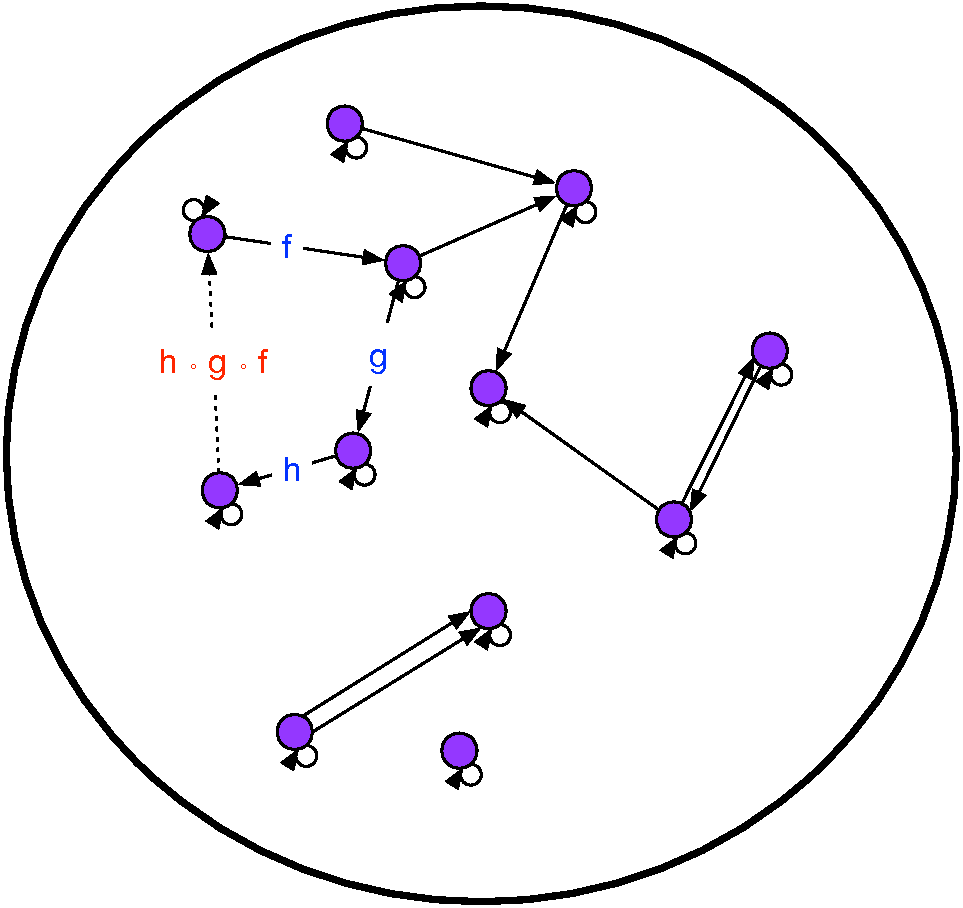
\includegraphics[width=.9\linewidth]{images/Category1.pdf}
\end{center}
\end{frame}
\begin{frame}[fragile,label=sec-12-3]{Not all sets}
Instead of sets with elements and functions, we have categories with objects
and morphisms.

\vspace{2ex}All sets are categories, but not vice-versa.
\end{frame}
\begin{frame}[fragile,label=sec-12-4]{Example: Any set}
\begin{description}[style=nextline]
  \item[Objects]   Set elements
  \item[Morphisms] Just the identities (a \textbf{discrete} category)
\end{description}
\end{frame}
\begin{frame}[fragile,label=sec-12-5]{Example: Posets}
\begin{description}[style=nextline]
  \item[Objects]     Set elements
  \item[Morphisms]   Identities and $≤$ between some elements
  \item[Composition] {\small $(y ≤ z) ∘ (x ≤ y) = (x ≤ z)$}
\end{description}
\end{frame}
\begin{frame}[fragile,label=sec-12-6]{Example: Graphs}
\begin{description}[style=nextline]
  \item[Objects]     Vertices
  \item[Morphisms]   Edges and self-edges (bidirectional if undirected)
  \item[Composition] In the ``obvious'' way.
\end{description}
\end{frame}
\begin{frame}[fragile,label=sec-12-7]{Example: Set}
\begin{description}[style=nextline]
  \item[Objects]     Sets
  \item[Morphisms]   Functions
  \item[Composition] As functions do
\end{description}
\end{frame}
\begin{frame}[fragile,label=sec-12-8]{Example: Mon}
\begin{description}[style=nextline]
  \item[Objects]     Sets with monoid structure
  \item[Morphisms]   Monoid homomorphisms
  \item[Composition] As functions do
\end{description}
\end{frame}
\begin{frame}[fragile,label=sec-12-9]{Example: Cat}
\begin{description}[style=nextline]
  \item[Objects]     Categories
  \item[Morphisms]   Functors
  \item[Composition] As functions do
\end{description}
\end{frame}
\begin{frame}[fragile,label=sec-12-10]{Example: Fun(C,D)}
\begin{description}[style=nextline]
  \item[Objects]     Functors $C → D$
  \item[Morphisms]   Natural transformations
  \item[Composition] As polymorphic functions
\end{description}
\end{frame}
\begin{frame}[fragile,label=sec-12-11]{Many categories}
Any book on category theory will have many more examples of categories than
these few.
\end{frame}
\begin{frame}[fragile,label=sec-12-12]{Some books}
\begin{itemize}
\item Lawvere, \emph{Conceptual Mathematics: A First Introduction to Categories}
\item Awodey, \emph{Category Theory}
\item Mac Lane, \emph{Categories for the Working Mathematician}
\end{itemize}
\end{frame}
\begin{frame}[fragile,label=sec-12-13]{Other resources}
\begin{itemize}
\item Catster's videos: \\
  \small \url{http://byorgey.wordpress.com/catsters-guide-2} \normalsize
\item Awodey's presentation on Category Theory at OPLSS 2013
\item \#\#categorytheory on IRC
\end{itemize}
\end{frame}
\begin{frame}[fragile,label=sec-12-14]{Concepts transfer}
One of the profound concepts in category theory is how ideas transfer.
\note{note
And yet, all of this is rooted in a profound simplicity.}
\end{frame}
\section{Functors}
\label{sec-13}
\begin{frame}[fragile,plain,label=sec-13-1]{HEAD}
\head{Functors}
\end{frame}
\begin{frame}[fragile,label=sec-13-2]{Categorical model}
\begin{center}
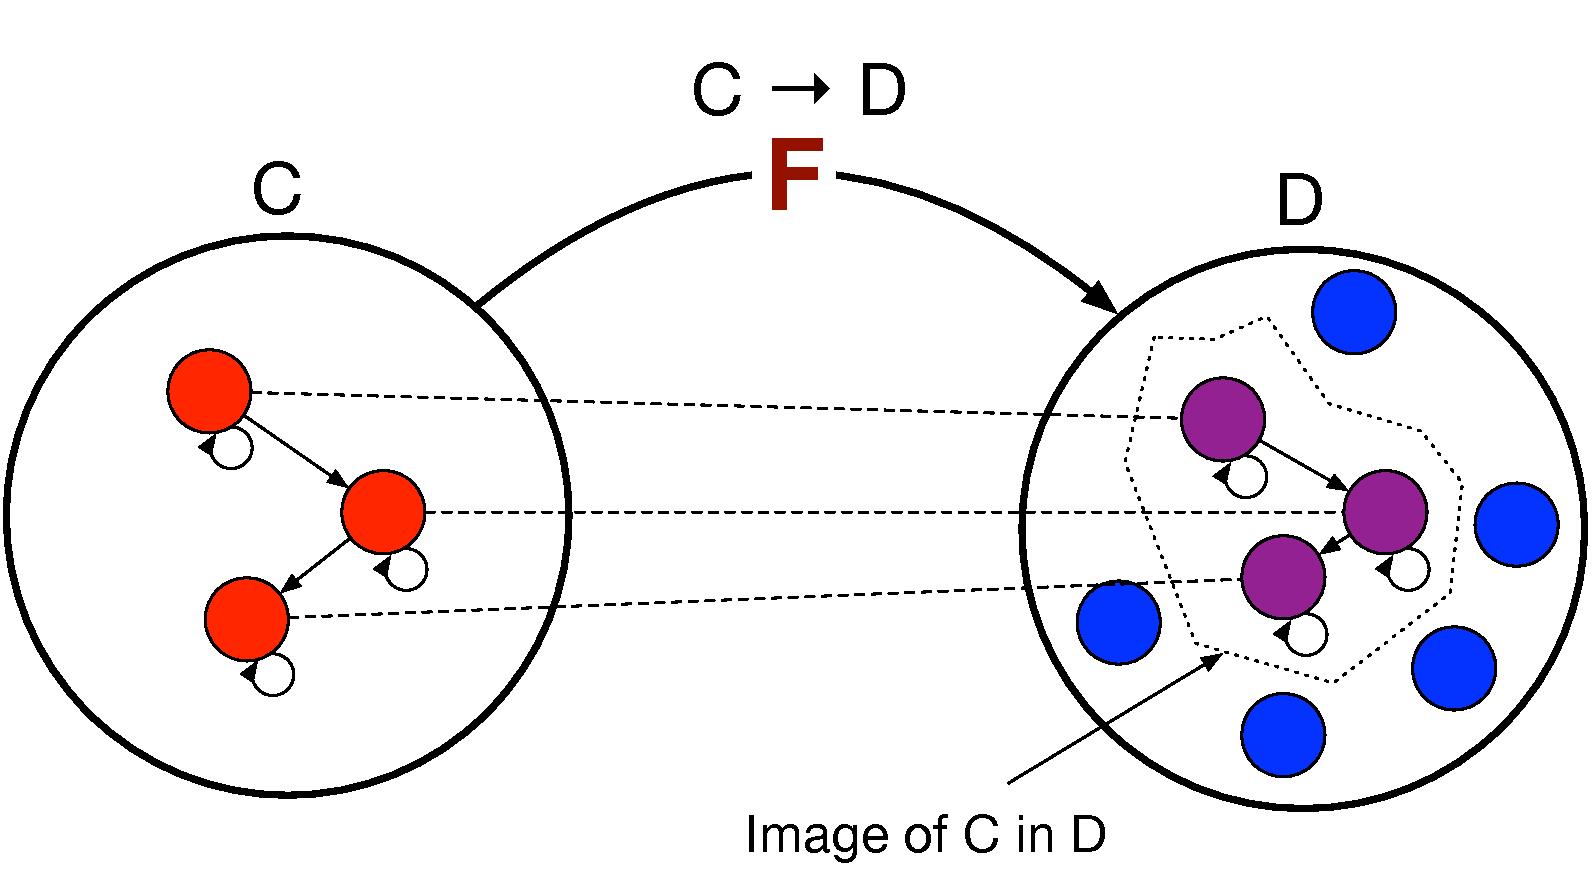
\includegraphics[width=\linewidth]{images/Functors1.pdf}
\end{center}
\end{frame}
\begin{frame}[fragile,label=sec-13-3]{Unit mapping}
\begin{center}
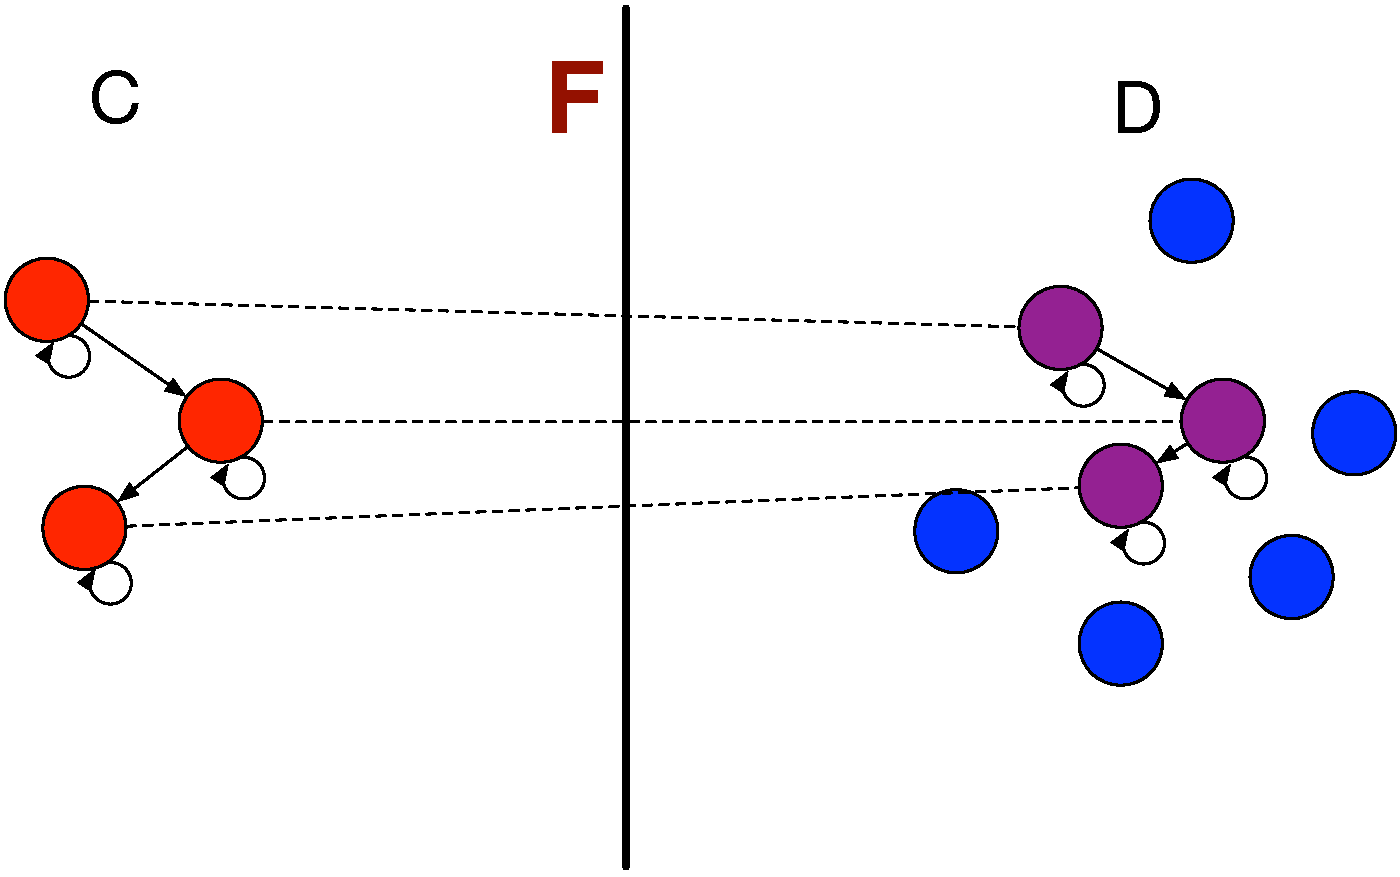
\includegraphics[width=\linewidth]{images/Functors2.pdf}
\end{center}
\note{note
In Haskell, this is called Const.}
\end{frame}
\begin{frame}[fragile,label=sec-13-4]{Definition in code}
\begin{lstlisting}[language=Haskell]
class Functor f where
  fmap :: (a -> b) -> (f a -> f b)
\end{lstlisting}
\end{frame}
\begin{frame}[fragile,label=sec-13-5]{Functor laws}
\begin{definition}[1. Identity law]
\( fmap\ id = id \)
\end{definition}
\begin{definition}<2->[2. Composition law]
\( fmap\ (f ∘ g) = fmap\ f ∘ fmap\ g \)
\end{definition}
\end{frame}
\begin{frame}[fragile,label=sec-13-6]{Not containers!}
A \alert{Functor} can sometimes map to:
\begin{itemize}
\item a container
\item a computation
\end{itemize}
\dots{}but a \alert{Functor} \emph{per se} is neither.
\end{frame}
\begin{frame}[fragile,label=sec-13-7]{As Context}
\fontsize{42}{48}\selectfont
\[ \textbf{F}\ {\tt a} \]
\end{frame}
\begin{frame}[fragile,label=sec-13-8]{Don't be fooled}
\alert{Functors} are humble, but powerful.
\end{frame}
\begin{frame}[fragile,label=sec-13-9]{Origins}
\begin{quotation} %% Eilenberg and Mac Lane
\noindent Their [Eilenberg and Mac Lane's] goal was to understand natural
transformations; in order to do that, functors had to be defined, which
required categories.

-- Wikipedia
\end{quotation}
\end{frame}
\begin{frame}[fragile,label=sec-13-10]{Identity}
\begin{lstlisting}[language=Haskell]
data Identity a = Identity a

instance Functor Identity where
  fmap f (Identity x) = ?
\end{lstlisting}
\note{note
Identity as a concept can be used to implement "taintedness", to force
laziness, to provide singletons, and more.  As should be clear by now, the
simplicity of a core idea can be misleading.}
\end{frame}
\begin{frame}[fragile,label=sec-13-11]{Identity}
\begin{lstlisting}[language=Haskell]
data Identity a = Identity a

instance Functor Identity where
  fmap f (Identity x)
    = Identity (f x)
\end{lstlisting}
\end{frame}
\begin{frame}[fragile,label=sec-13-12]{Proving Identity Law}
\fontsize{12}{16}\selectfont
\begin{align*}
id\ {\tt x}              &= fmap\ id\ {\tt x}                      \\
                         &                                         \\
id\ ({\tt Identity\ x′}) &= fmap\ id\ ({\tt Identity\ x′})
                            \tag*{\textbf{unfold {\tt x}}}         \\
                         &= {\tt Identity}\ (id\ {\tt x′})
                            \tag*{\textbf{defn. {\tt fmap}}}       \\
{\tt Identity\ x′}       &= {\tt Identity\ x′}
                            \tag*{\textbf{defn. {\tt id}}}
\end{align*}
\end{frame}
\begin{frame}[fragile,label=sec-13-13]{Proving Composition}
\fontsize{12}{16}\selectfont
\begin{align*}
 &  \hspace{1.3em}fmap\ (f ∘ g)\ {\tt x}             \\
 &= fmap\ (f ∘ g)\ ({\tt Identity\ x′})
    \tag*{\textbf{unfold {\tt x}}}                   \\
 &= {\tt Identity}\ ((f ∘ g)\ {\tt x′})
    \tag*{\textbf{defn. {\tt fmap}}}                 \\
 &= {\tt Identity}\ (f (g ({\tt x′})))
    \tag*{\textbf{defn. ∘}}                          \\
 &= fmap\ f\ ({\tt Identity} (g ({\tt x′})))
    \tag*{\textbf{defn. {\tt fmap}}}                 \\
 &= fmap\ f\ (fmap\ g\ ({\tt Identity\ x′}))
    \tag*{\textbf{defn. {\tt fmap}}}                 \\
 &= fmap\ f\ (fmap\ g\ {\tt x})
    \tag*{\textbf{fold {\tt x}}}
\end{align*}
\end{frame}
\begin{frame}[fragile,label=sec-13-14]{Maybe}
\begin{lstlisting}[language=Haskell]
data Maybe a = Nothing | Just a

instance Functor Maybe where
  fmap f Nothing  = ?
  fmap f (Just x) = ?
\end{lstlisting}
\end{frame}
\begin{frame}[fragile,label=sec-13-15]{Maybe}
\begin{lstlisting}[language=Haskell]
data Maybe a = Nothing | Just a

instance Functor Maybe where
  fmap f Nothing  = Nothing
  fmap f (Just x) = Just (f x)
\end{lstlisting}
\end{frame}
\begin{frame}[fragile,label=sec-13-16]{Either}
\begin{lstlisting}[language=Haskell]
data Left e a = Left e | Right a
\end{lstlisting}
\end{frame}
\begin{frame}[fragile,label=sec-13-17]{Tuple}
\begin{lstlisting}[language=Haskell]
data Pair p a = Pair p a
\end{lstlisting}
\end{frame}
\begin{frame}[fragile,label=sec-13-18]{Const}
\begin{lstlisting}[language=Haskell]
data Const c a = Const c
\end{lstlisting}
\end{frame}
\begin{frame}[fragile,label=sec-13-19]{Exercise}
Remember how free functors were encoded as functions?  This extends to \alert{any}
functor:

\[ f\ a \ ≅ \ ∀ r, (a → r) → f\ r \]
\end{frame}
\begin{frame}[fragile,label=sec-13-20]{Exercise}
\fontsize{14}{16}\selectfont
\vspace{-2ex}
\begin{align*}
\texttt{lower} & \ :: \ (∀ r.\ (a → r) → f\ r) \ → \ f\ a                    \\[1ex]
\texttt{lift}  & \ :: \ \texttt{Functor}\ f \ ⇒ \ f\ a \ → \ (a → r) → f\ r
\end{align*}
\end{frame}
\begin{frame}[fragile,label=sec-13-21]{Yoneda lemma}
You just proved the Yoneda lemma in a functional language!
\end{frame}
\begin{frame}[fragile,label=sec-13-22]{Exercise}
A Yoneda embedding is itself a \alert{Functor}:

\vspace{2ex}
\lstset{basicstyle=\footnotesize\ttfamily}
\begin{lstlisting}[language=Haskell]
data Yoneda f a
  = Yoneda (forall r. (a -> r) -> f r)

instance Functor (Yoneda f) where
  fmap g (Yoneda k) = ?
\end{lstlisting}
\end{frame}
\begin{frame}[fragile,label=sec-13-23]{fmap optimization}
One thing Yoneda buys us (among others) is optimization of repeated calls to
\texttt{fmap}.
\note{note
Identity as a concept can be used to implement "taintedness", to force
laziness, to provide singletons, and more.  As should be clear by now, the
simplicity of a core idea can be misleading.}
\end{frame}
\begin{frame}[fragile,label=sec-13-24]{Concepts lift}
A lot of what we know about values can be lifted to functors.
\end{frame}
\begin{frame}[fragile,label=sec-13-25]{Lifted Identity}
\begin{lstlisting}[language=Haskell]
data IdentityF f a
  = IdentityF (f a)
\end{lstlisting}
\end{frame}
\begin{frame}[fragile,label=sec-13-26]{Lifted Maybe}
\begin{lstlisting}[language=Haskell]
data MaybeF f a
  = NothingF a | Just (f a)
\end{lstlisting}
\end{frame}
\begin{frame}[fragile,label=sec-13-27]{Lifted Either}
\begin{lstlisting}[language=Haskell]
data EitherF f g a
  = LeftF (f a) | RightF (g a)
\end{lstlisting}
\end{frame}
\begin{frame}[fragile,label=sec-13-28]{Lifted Tuple}
\begin{lstlisting}[language=Haskell]
data TupleF f g a
  = TupleF (f (g a))
\end{lstlisting}
\end{frame}
\begin{frame}[fragile,label=sec-13-29]{Lifted List}
\begin{lstlisting}[language=Haskell]
data ListF f a
  = NilF a
  | ListF (f (ListF f a))
\end{lstlisting}
\end{frame}
\begin{frame}[fragile,label=sec-13-30]{Free Monad}
We could rename the constructors of our lifted list:

\vspace{2ex}
\begin{lstlisting}[language=Haskell]
data FreeMonad m a
  = Return a
  | Join (m (FreeMonad m a))
\end{lstlisting}
\end{frame}
\begin{frame}[fragile,label=sec-13-31]{As Context}
\fontsize{42}{48}\selectfont
\[ \textbf{F}\ {\tt a} \]
\end{frame}
\begin{frame}[fragile,label=sec-13-32]{As Context}
\fontsize{32}{36}\selectfont
\[ \textbf{[F]}\ {\tt a} \]
\end{frame}
\begin{frame}[fragile,label=sec-13-33]{As Context}
\fontsize{32}{36}\selectfont
\[ \textbf{[]}\ {\tt a} \]
\fontsize{14}{16}\selectfont
\begin{example}[\vspace*{-3.5ex}]
\begin{lstlisting}[language=Haskell]
  Return a
\end{lstlisting}
\end{example}
\end{frame}
\begin{frame}[fragile,label=sec-13-34]{As Context}
\fontsize{32}{36}\selectfont
\[ \textbf{[F, F, F]}\ {\tt a} \]
\fontsize{14}{16}\selectfont
\begin{example}[\vspace*{-3.5ex}]
\begin{lstlisting}[language=Haskell]
  Join
    (f (Join
        (f (Join
            (f (Return a))))))
\end{lstlisting}
\end{example}
\end{frame}
\begin{frame}[fragile,label=sec-13-35]{Famous quote}
\begin{quotation}
\noindent ``A monad is just a monoid in the category of endofunctors, what's the
problem?'' \\
-- Saunders Mac Lane
\end{quotation}

\vspace{2ex}Likewise, our free monad is just a free monoid over functors.
\note{note
We're not going to discuss this just now, but we're going to come back it.}
\end{frame}
\section{[Break]}
\label{sec-14}
\begin{frame}[fragile,label=sec-14-1]{[Break]}
\begin{center}

\includegraphics[width=.9\linewidth]{images/monad-tutorial.jpg}
\end{center}
\end{frame}
\section{Applicatives}
\label{sec-15}
\begin{frame}[fragile,plain,label=sec-15-1]{HEAD}
\head{Applicatives}
\end{frame}
\begin{frame}[fragile,label=sec-15-2]{Definition in code}
\begin{lstlisting}[language=Haskell]
class Functor f
    => Applicative f where
  pure  :: f a
  (<*>) :: f (a -> b) -> f a -> f b
\end{lstlisting}
\end{frame}
\begin{frame}[fragile,label=sec-15-3]{Important}
One aspect of \texttt{Applicative} gives a clue to its power:

\vspace{2ex}The \texttt{<*>} operator takes \alert{two} functorial arguments.
\note{note
This is not true of either Functor or Monad.}
\end{frame}
\begin{frame}[fragile,label=sec-15-4]{Applicative laws}
\begin{definition}[1. Identity law]
\( pure\ id ⊗ v = v \)
\end{definition}
\begin{definition}<2->[2. Composition law]
\( pure\ (∘) ⊗ u ⊗ v ⊗ w = u ⊗ (v ⊗ w) \)
\end{definition}
\begin{definition}<3->[3. Homomorphism law]
\( pure\ f ⊗ pure\ x = pure\ (f(x)) \)
\end{definition}
\end{frame}
\begin{frame}[fragile,label=sec-15-5]{Applicative laws}
\begin{definition}[4. Interchange law]
\( u ⊗ pure\ y = pure\ (\$\ y) ⊗ u \)
\end{definition}
\begin{definition}<2->[5. Functor relation law]
\( pure\ f ⊗ x = fmap\ f\ x \)
\end{definition}
\end{frame}
\begin{frame}[fragile,label=sec-15-6]{Identity}
\begin{lstlisting}[language=Haskell]
data Identity a = Identity a

instance Applicative Identity where
  pure x = Identity x
  Identity f <*> Identity x = ?
\end{lstlisting}
\end{frame}
\begin{frame}[fragile,label=sec-15-7]{Identity}
\begin{lstlisting}[language=Haskell]
data Identity a = Identity a

instance Applicative Identity where
  pure x = Identity x
  Identity f <*> Identity x
    = Identity (f x)
\end{lstlisting}
\end{frame}
\begin{frame}[fragile,label=sec-15-8]{Proving Identity}
\fontsize{12}{16}\selectfont
\begin{align*}
 &  \hspace{1.3em}pure\ id ⊗ {\tt v}                 \\
 &= pure\ id ⊗ {\tt Identity\ v}
    \tag*{\textbf{unfold {\tt v}}}                   \\
 &= {\tt Identity}\ id ⊗ {\tt Identity\ v}
    \tag*{\textbf{defn. {\tt pure}}}                 \\
 &= {\tt Identity}\ (id\ {\tt v})
    \tag*{\textbf{defn. ⊗}}                          \\
 &= {\tt Identity\ v}
    \tag*{\textbf{defn. {\tt id}}}                   \\
 &= {\tt v}
    \tag*{\textbf{fold {\tt v}}}
\end{align*}
\end{frame}
\begin{frame}[fragile,label=sec-15-9]{Proving Homomorphism}
\fontsize{12}{16}\selectfont
\begin{align*}
 &  \hspace{1.3em}pure\ f ⊗ pure\ x                  \\
 &= {\tt Identity}\ f ⊗ {\tt Identity}\ x
    \tag*{\textbf{defn. {\tt pure}}}                 \\
 &= {\tt Identity}\ (f(x))
    \tag*{\textbf{defn. ⊗}}                          \\
 &= pure\ (f(x))
    \tag*{\textbf{defn. {\tt pure}}}
\end{align*}
\end{frame}
\begin{frame}[fragile,label=sec-15-10]{Maybe}
\begin{lstlisting}[language=Haskell]
data Maybe a = Nothing | Just a

instance Applicative Maybe where
  pure x = ?

  Nothing <*> Nothing = ?
  Just f  <*> Nothing = ?
  Nothing <*> Just x  = ?
  Just f  <*> Just x  = ?
\end{lstlisting}
\end{frame}
\begin{frame}[fragile,label=sec-15-11]{Maybe}
\begin{lstlisting}[language=Haskell]
data Maybe a = Nothing | Just a

instance Applicative Maybe where
  pure x = ?

  Just f <*> Just x = Just (f x)
  _      <*> _      = Nothing
\end{lstlisting}
\end{frame}
\begin{frame}[fragile,label=sec-15-12]{Either}
\begin{lstlisting}[language=Haskell]
data Left e a = Left e | Right a
\end{lstlisting}
\end{frame}
\begin{frame}[fragile,label=sec-15-13]{Tuple}
\begin{lstlisting}[language=Haskell]
data Pair p a = Pair p a
\end{lstlisting}
\end{frame}
\begin{frame}[fragile,label=sec-15-14]{Const}
\alert{Const} requires a trickier instance.
\begin{example}[\vspace*{-3.5ex}]
\begin{lstlisting}[language=Haskell]
data Const c a = Const c

instance Monoid c
    => Applicative (Const c) where
  pure x = ?
  Const a <*> Const b = ?
\end{lstlisting}
\end{example}
\end{frame}
\begin{frame}[fragile,label=sec-15-15]{Analysis}
Applicatives allow for expression analysis.

\vspace{2ex}\textbf{Example}: Minimizing expensive key lookups.
\end{frame}
\begin{frame}[fragile,label=sec-15-16]{Composition}
Another useful trait is that applicatives compose well.

\fontsize{14}{16}\selectfont
\vspace{2ex}\url{http://comonad.com/reader/2012/abstracting-with-applicatives}
\end{frame}
\section{Monads}
\label{sec-16}
\begin{frame}[fragile,plain,label=sec-16-1]{HEAD}
\head{Monads}
\end{frame}
\begin{frame}[fragile,label=sec-16-2]{Definition in code}
\begin{lstlisting}[language=Haskell]
class Monad m where
  return :: m a
  (>>=)  :: m a -> (a -> m b) ->
            m b
\end{lstlisting}
\note{note
And this is all that monads are!}
\end{frame}
\begin{frame}[fragile,label=sec-16-3]{Definition in code (join)}
\begin{lstlisting}[language=Haskell]
class Monad m where
  return :: m a
  join   :: m (m a) -> m a
\end{lstlisting}
\end{frame}
\begin{frame}[fragile,label=sec-16-4]{Bind in terms of join}
\begin{example}[\vspace*{-3.5ex}]
\begin{lstlisting}[language=Haskell]
    m >>= f  =  join (fmap f m)
\end{lstlisting}
\end{example}
\end{frame}
\begin{frame}[fragile,label=sec-16-5]{How bind works}
\begin{example}[\vspace*{-3.5ex}]
\begin{lstlisting}[language=Haskell]
             m  :: m a
           f    ::   a -> m b
      fmap f    :: m a -> m (m b)
      fmap f m  :: m (m b)
join (fmap f m) :: m b
\end{lstlisting}
\end{example}
\end{frame}
\begin{frame}[fragile,label=sec-16-6]{Not fmap}
Differs from fmap in that a new \texttt{m} was created.
\end{frame}
\begin{frame}[fragile,label=sec-16-7]{Monad laws}
\begin{definition}[1. Left identity law]
\( \texttt{return}\ a\ \text{\texttt{\normalsize >>=}}\ f \color{red}=\color{black} f\ a \)
\end{definition}
\begin{definition}<2->[2. Right identity Law]
\( m \ \text{\texttt{\normalsize >>=}}\ \texttt{return} \color{red}=\color{black} m \)
\end{definition}
\begin{definition}<3->[3. Associativity Law]
\( (m \ \text{\texttt{\normalsize >>=}}\ f) \ \text{\texttt{\normalsize >>=}}\ g \color{red}=\color{black}
    m \ \text{\texttt{\normalsize >>=}}\ λx → f\ x \ \text{\texttt{\normalsize >>=}}\ g \)
\end{definition}
\end{frame}
\begin{frame}[fragile,label=sec-16-8]{Monadic composition}
\begin{example}[\vspace*{-3.5ex}]
\lstset{keywordstyle=\color{black}}
\begin{lstlisting}[language=Haskell]
f >=> g  =  \x -> f x >>= g

g <=< f  =  \x -> g =<< f x
\end{lstlisting}
\end{example}
\end{frame}
\begin{frame}[fragile,label=sec-16-9]{Monad laws (form 2)}
\begin{definition}[1. Left identity law (alt)]
\( \texttt{return}\ \text{\texttt{\small >=>}}\ f \color{red}=\color{black} f \)
\end{definition}
\begin{definition}<2->[2. Right identity Law (alt)]
\( f\ \text{\texttt{\small >=>}}\ \texttt{return} \color{red}=\color{black} f \)
\end{definition}
\begin{definition}<3->[3. Associativity Law (alt)]
\( (f\ \text{\texttt{\small >=>}}\ g)\ \text{\texttt{\small >=>}}\ h \color{red}=\color{black} f\ \text{\texttt{\small >=>}}\ (g\ \text{\texttt{\small >=>}}\ h) \)
\end{definition}
\end{frame}
\begin{frame}[fragile,label=sec-16-10]{Chaining}
Monads allow us to chain computations.
\begin{example}[\vspace*{-3.5ex}]
\begin{lstlisting}[language=Haskell]
x >>= f >>= g >>= >>= h
\end{lstlisting}
\end{example}
\end{frame}
\begin{frame}[fragile,label=sec-16-11]{Chaining}
Haskell has a special notation for this:
\begin{example}[\vspace*{-3.5ex}]
\begin{lstlisting}[language=Haskell]
do a <- x
   b <- f a
   c <- g b
   h c
\end{lstlisting}
\end{example}
\end{frame}
\begin{frame}[fragile,label=sec-16-12]{Desugared}
This is just sugar for:
\begin{example}[\vspace*{-3.5ex}]
\begin{lstlisting}[language=Haskell]
  (x   >>= \a ->
   f a >>= \b ->
   g b >>= \c ->
   h c)
\end{lstlisting}
\end{example}
\end{frame}
\begin{frame}[fragile,label=sec-16-13]{Thinking about join}
When implementing a new Monad, ask yourself: What does it mean to ``multiply''
two contexts?
\end{frame}
\begin{frame}[fragile,label=sec-16-14]{Identity}
\begin{lstlisting}[language=Haskell]
data Identity a = Identity a

instance Functor Identity where
  Identity m >>= f = ?
\end{lstlisting}
\note{note
Identity as a concept can be used to implement "taintedness", to force
laziness, to provide singletons, and more.  As should be clear by now, the
simplicity of a core idea can be misleading.}
\end{frame}
\begin{frame}[fragile,label=sec-16-15]{Identity}
\begin{lstlisting}[language=Haskell]
data Identity a = Identity a

instance Functor Identity where
  Identity m >>= f = f m
\end{lstlisting}
\end{frame}
\begin{frame}[fragile,label=sec-16-16]{Proving Left Identity}
\fontsize{14}{17}\selectfont
\begin{align*}
 &  \hspace{1.3em}return\ {\tt a} >>= f              \\
 &= {\tt Identity\ a} >>= f
    \tag*{\textbf{defn. {\tt return}}}               \\
 &= f\ {\tt a}
    \tag*{\textbf{defn. {\tt >>=}}}
\end{align*}
\end{frame}
\begin{frame}[fragile,label=sec-16-17]{Proving Right Identity}
\fontsize{14}{17}\selectfont
\begin{align*}
 &  \hspace{1.3em}{\tt m} >>= return                 \\
 &= {\tt Identity\ m′} >>= return
    \tag*{\textbf{unfold {\tt m}}}                   \\
 &= return\ {\tt m′}
    \tag*{\textbf{defn. {\tt >>=}}}                  \\
 &= {\tt Identity\ m′}
    \tag*{\textbf{defn. {\tt return}}}               \\
 &= {\tt m}
    \tag*{\textbf{fold {\tt m}}}
\end{align*}
\end{frame}
\begin{frame}[fragile,label=sec-16-18]{Proving Associativity}
\fontsize{12}{16}\selectfont
\begin{align*}
 &  \hspace{1.3em}(m >>= f) >>= g                    \\
 &= ({\tt Identity\ m′} >>= f) >>= g
    \tag*{\textbf{unfold {\tt m}}}                   \\
 &= f\ {\tt m′} >>= g
    \tag*{\textbf{defn. {\tt >>=}}}                  \\
 &= (λx → f\ x >>= g)\ {\tt m′}
    \tag*{\textbf{η-expansion}}                      \\
 &= {\tt Identity\ m′} >>= (λx → f\ x >>= g)
    \tag*{\textbf{defn. {\tt >>=}}}                  \\
 &= m >>= (λx → f\ x >>= g)
    \tag*{\textbf{fold {\tt m}}}
\end{align*}
\end{frame}
\begin{frame}[fragile,label=sec-16-19]{Maybe}
\begin{lstlisting}[language=Haskell]
data Maybe a = Nothing | Just a

instance Functor Maybe where
  Nothing >>= f = ?
  Just x  >>= f = ?
\end{lstlisting}
\end{frame}
\begin{frame}[fragile,label=sec-16-20]{Maybe}
\begin{lstlisting}[language=Haskell]
data Maybe a = Nothing | Just a

instance Functor Maybe where
  Nothing >>= f = Nothing
  Just x  >>= f = Just (f x)
\end{lstlisting}
\end{frame}
\begin{frame}[fragile,label=sec-16-21]{Maybe}
\texttt{Maybe} gives us a way to short-circuiting a chain of computations.
\end{frame}
\begin{frame}[fragile,label=sec-16-22]{Either}
\begin{lstlisting}[language=Haskell]
data Left e a = Left e | Right a
\end{lstlisting}
\end{frame}
\begin{frame}[fragile,label=sec-16-23]{Either}
\texttt{Either} lets us short-circuit with an alternate result.
\end{frame}
\begin{frame}[fragile,label=sec-16-24]{Tuple}
What additional constraint is needed to make this a Monad, and why?
\begin{example}[\vspace*{-3.5ex}]
\begin{lstlisting}[language=Haskell]
data Pair w a = Pair w a
\end{lstlisting}
\end{example}
\end{frame}
\begin{frame}[fragile,label=sec-16-25]{Tuple}
Tuples form the Writer monad, if we write one more function:
\begin{example}[\vspace*{-3.5ex}]
\begin{lstlisting}[language=Haskell]
tell :: w -> Pair w ()
tell w = ?
\end{lstlisting}
\end{example}
\end{frame}
\begin{frame}[fragile,label=sec-16-26]{Exercise: Const}
Why can't it be a monad?
\note{note
Because Const (Const a) does not preserve the value from the inner Const.}
\end{frame}
\begin{frame}[fragile,label=sec-16-27]{Reader}
Functions are functors, applicatives and monads too.  As a monad, it's often
called \texttt{Reader}.
\begin{example}[\vspace*{-3.5ex}]
\begin{lstlisting}[language=Haskell]
instance Monad ((->) a) where
  return x = ?
  k >>= f  = ?
\end{lstlisting}
\end{example}
\end{frame}
\begin{frame}[fragile,label=sec-16-28]{State}
\texttt{State} is prototypical of what monads are about.
\begin{example}[\vspace*{-3.5ex}]
\begin{lstlisting}[language=Haskell]
newtype State s a
  = State { runS :: s -> (a, s) }

instance Monad (State s) where
  return x = ?
  k >>= f  = ?
\end{lstlisting}
\end{example}
\end{frame}
\begin{frame}[fragile,label=sec-16-29]{State}
\texttt{State} is made useful by two more functions, \texttt{put} and
\texttt{get}.
\begin{example}[\vspace*{-3.5ex}]
\begin{lstlisting}[language=Haskell]
put :: s -> State s ()
put s = ?

get :: State s s
get = ?
\end{lstlisting}
\end{example}
\end{frame}
\begin{frame}[fragile,label=sec-16-30]{Silly example}
\begin{example}[\vspace*{-3.5ex}]
\begin{lstlisting}[language=Haskell]
let f x = when (even x) $ do
        y <- get
        put (x + y)
in flip execState 0 $
   mapM_ f [1,2,3,4,5]
\end{lstlisting}
\end{example}
\end{frame}
\begin{frame}[fragile,label=sec-16-31]{Free Monads}
With free monads, we can defer the choice of return and bind, allowing us to
model computations.
\end{frame}
\section{The End}
\label{sec-17}
\begin{center}

\includegraphics[width=\linewidth]{images/this-meeting-is-over_3.jpg}
\end{center}
\section{Colophon}
\label{sec-18}
% Emacs 24.3.1 (Org mode 8.2.6)
\end{document}